\documentclass[11pt]{article}
%%% PAGE DIMENSIONS
\usepackage{geometry} % to change the page dimensions
\geometry{a4paper} % or letterpaper (US) or a5paper or....
\geometry{margin=1.5in, left=0.75in, right=0.75in, headheight = 14pt} % for example, change the margins to 2 inches all round
% \geometry{landscape} % set up the page for landscape
%   read geometry.pdf for detailed page layout information
\usepackage{graphicx} % support the \includegraphics command and options
\usepackage{longtable}
\usepackage{float}
\usepackage{wrapfig}
\usepackage{multicol}
\usepackage{multirow}
\usepackage[normalem]{ulem}
\useunder{\uline}{\ul}{}
\usepackage[table,xcdraw]{xcolor}

\usepackage[parfill]{parskip} % Activate to begin paragraphs with an empty line rather than an indent

%%% PACKAGES
\usepackage{booktabs} % for much better looking tables
\usepackage{array} % for better arrays (eg matrices) in maths
\usepackage{paralist} % very flexible & customisable lists (eg. enumerate/itemize, etc.)
\usepackage{verbatim} % adds environment for commenting out blocks of text & for better verbatim
\usepackage{subfig} % make it possible to include more than one captioned figure/table in a single float
% These packages are all incorporated in the memoir class to one degree or another...

\usepackage{listings}

%%% TITLE AND AUTHOR

\title{ 
    Biologically Inspired Computation
}

\author{Nathan Billis}
%\date{} % Activate to display a given date or no date (if empty),
         % otherwise the current date is printed 
\makeatletter

%%% HEADERS & FOOTERS
\usepackage{fancyhdr} % This should be set AFTER setting up the page geometry
\pagestyle{fancy} % options: empty , plain , fancy
\renewcommand{\headrulewidth}{1pt} % customise the layout...
\lhead{\@title}\chead{}\rhead{\@author}
\lfoot{}\cfoot{\thepage}\rfoot{}


%%% SECTION TITLE APPEARANCE
\usepackage{sectsty}
\allsectionsfont{\sffamily\mdseries\upshape} % (See the fntguide.pdf for font help)
% (This matches ConTeXt defaults)

%%% ToC (table of contents) APPEARANCE
\usepackage[nottoc,notlof,notlot]{tocbibind} % Put the bibliography in the ToC
\usepackage[titles,subfigure]{tocloft} % Alter the style of the Table of Contents
\renewcommand{\cftsecfont}{\rmfamily\mdseries\upshape}
\renewcommand{\cftsecpagefont}{\rmfamily\mdseries\upshape} % No bold!

% biblatex for citations
\usepackage{csquotes}
\usepackage[backend=biber,citestyle=ieee]{biblatex}
\addbibresource{references.bib}
\usepackage{url}

\usepackage[colorlinks=false,
            allbordercolors={0 0 0},
            pdfborderstyle={/S/U/W 1}]{hyperref}


\graphicspath{{images/}}

\begin{document}
\begin{titlepage}
    \centering
    {\scshape\LARGE Department of Electronics \par}
    \vspace{1cm}
    {\scshape\Large Biologically Inspired Computing \par}
    \vspace{1cm}
    {\scshape\Large Top Three uses of Neural Networks in Voice Research \par}
    % maybe an image here
    \vfill
    {\Large\itshape \@author \par}
    \vspace{2cm}
    
    \tableofcontents

\end{titlepage}
\pagenumbering{arabic} % Start arabic numbering
	
\newpage

    \section{Introduction}
    
    Voice research is currently a very important research area, especially with the rise of smart speakers such as the Amazon Echo \cite{IntroducingRoom}, Google Nest \cite{GoogleStore} and Apple Homepod \cite{HomePodUK}. The importance of accurate voice recognition is not only important from an accessibility standpoint but also for people using these devices. 
    
    Speech has been an important way of communicating with each other and although speech recognition has moved alot very quickly it's still not perfect. When working with speech there are a variety of different issues. Some of the most common issues include \cite{Gevaert2010NeuralRecognition}: 
    \begin{itemize}
        \item Speaker Variation: where the same words are pronounced differently by diff rent people because of variations with gender, age, speed of speech and many other tiny changes.
        \item Background Noise: where the event is noisy it can add to the signal and even the speaker can add unwanted noise to the signal.
        \item Continuous Speech: when we speech there are occasions where there are no breaks between words making it difficult to disguise the start and ends of words.
        \item Other External Factors: in addition to the issues above there can be a variety of other factors such as the position of the microphone all having a knock on effect on the quality of the recording.
    \end{itemize}
    
    This report will look at why Automatic Speech Recognition, Large Vocabulary Speech Recognition, and Noise Robust Speech Recognition are the top three applications of neural networks within voice research.
    
    \section{Neural Networks Overview}
    Neural networks are the most common form of biologically inspired computing in the real world. There are many types of Neural Networks each having their own advantages and disadvantages. Many are treated as a black box style model with inputs on one side and outputs on the other, and they all generally require alot of training to present good results.
    
    \begin{figure}[h]
        \centering
        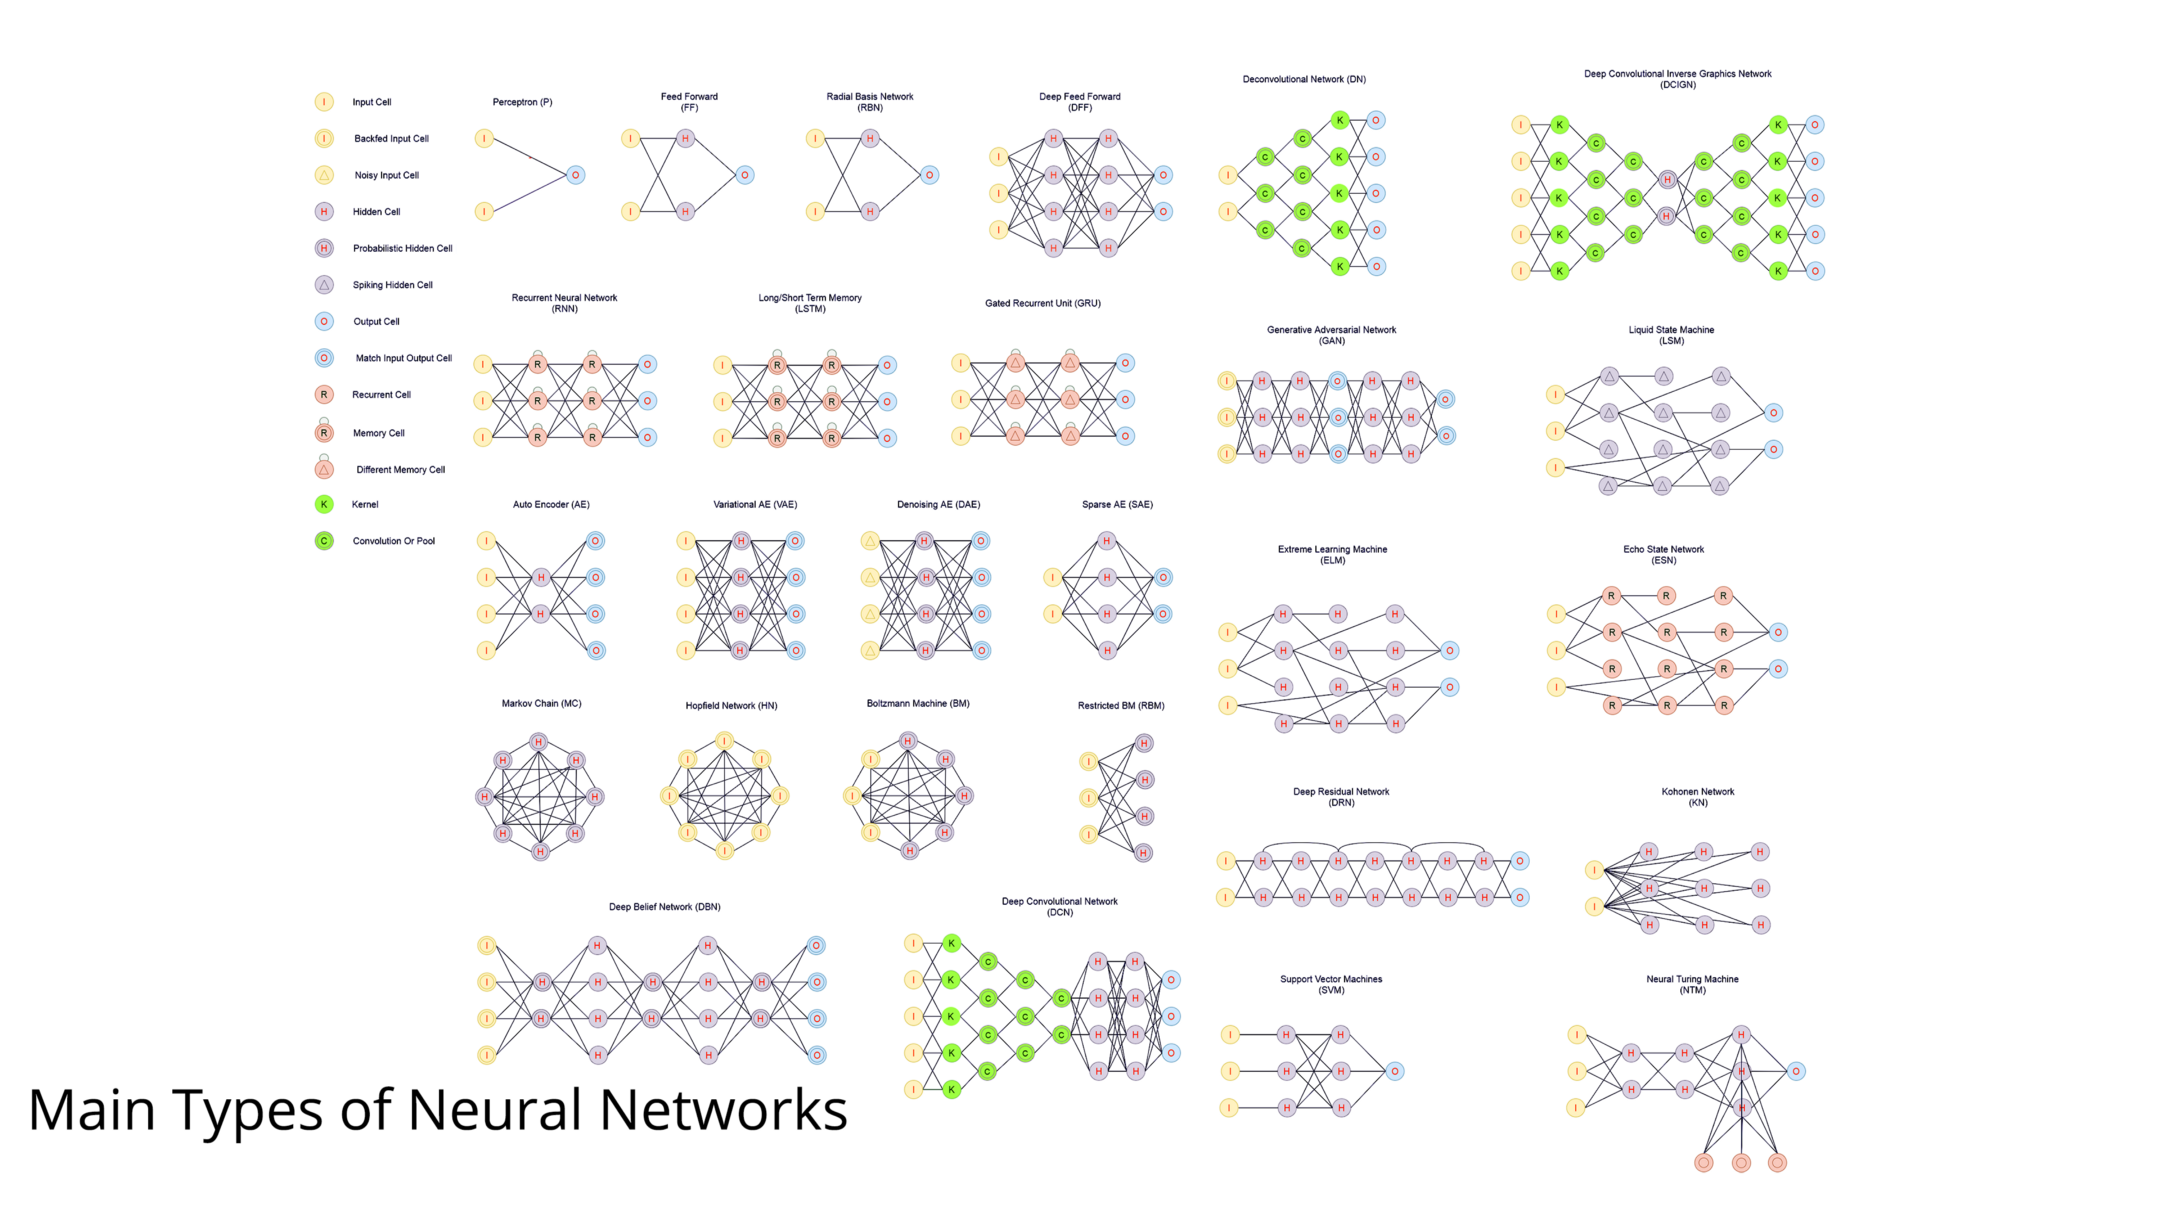
\includegraphics[scale=0.25]{neuralnetworks.png}
        \caption{Main Types of Neural Networks \cite{MainAI}}
        \label{fig:neuralNetworks}
    \end{figure}
    
    Figure \ref{fig:neuralNetworks} displays some of the popular neural network types. Each network has differing strengths and because of this they're adapted for their differing uses. The two main networks that are used in voice research are Feed Forward (FF) and Recurrent Neural Network (RNN), other types of networks are used however these two are the main one's we'll be focusing on. Neural Networks are made up of connected processes called neurons \cite{Schmidhuber2015DeepOverview}, each being activated in different ways with input nodes being activated by the environment. The complexity of the problem changes how many computational stages there needs to be in the network.
    
    \subsection{Feed Forward}
    Feed forward networks are arranged in layers \cite{NeuralArchitecture}, with each layer leading to the next layer and then onto the output. Unlike other forms of neural networks there are no connections between layers. The connection between each layer has differing weights and bias changing the result of the output.
    
    \subsection{Recurrent Neural Networks}
    
    
    
    
    
    
    \section{Automatic Speech Recognition (ASR)}
    


    \section{Large Vocabulary Speech Recognition}
    
    \section{Noise Robust Speech Recognition}
    
    \section{Conclusion}

        


\pagebreak

\printbibliography


\end{document}